
\section{Methodology}

We propose the following workflow for studying software evolution via VCS
data.  First, each version of all source files in the project are
reconstituted from the differences stored within the VCS such that each
version of a file can be parsed by an appropriate language front end.  Each
front-end is configured to map the parsed code to an annotated term (or,
aterm)~\cite{brand00aterm} that represents a standardized serialization of the
parse tree or abstract syntax tree.  Mapping languages to a common aterm
format allows the downstream portions of our workflow to be language-agnostic
to a large degree, with minimal language-specific parameterization.

\begin{figure}
\begin{center}
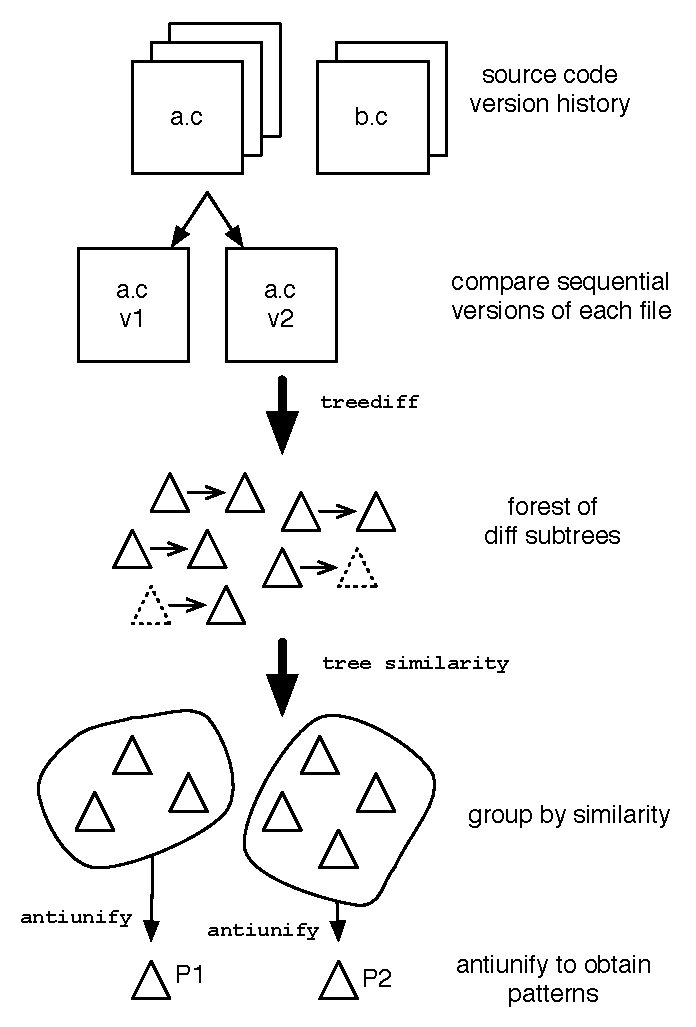
\includegraphics[height=0.44\textheight]{figures/workflow.pdf}
\caption{workflow}
\label{fig:workflow}
\end{center}
\end{figure}

Once we have code in an aterm format, we can then apply a structural
differencing algorithm between adjacent versions of each source file (e.g.,
version $n$ of file $f$ is compared to version $n+1$ of file $f$).  The result
of this is a forest of trees that represent the portions of the AST of file
$f$ that changed between versions at the structural level.  These changes can
either be code insertions, deletions, or mutations.  Our differencing is based
on the work of Yang~\cite{yang91diff} whose algorithm was designed for
computing differences between source code versions.  Yang's goal was to
improve the visual presentation of differences in textual diff tools, and our
use of their algorithm to provide input to further tree analysis algorithms is
novel.

After reducing the sequence of differences stored in the VCS, we have a large
forest of trees each representing a change that occurred over the evolution of
the software.  At this point, we seek to relate each of these trees via a
tree similarity metric.  This is achieved by using Yang's algorithm a second
time, but in this case we ignore the sequence of edit operations that it
produces and simply consume the quantitative similarity metric that it
produces as a rough estimate of how closely related two trees are.  A
threshold parameter is defined in which two trees with a similarity above the
threshold are considered to be part of the same group of difference tress.

Finally, once the set of differences are grouped into groups of trees that are
similar up to the threshold, we perform antiunification on the entire group to
distill all members to a representative code pattern for the group.  The
antiunification algorithm as described by Bulychev~\cite{bulychev08dupe} as
part of the clonedigger
project\footnote{\url{http://clonedigger.sourceforge.net}} was used, which
itself is an implementation of the classical antiunitification algorithm of
Reynolds~\cite{reynolds69antiunification}.

In the following sections, we descibe the steps above in greater detail.

\subsection{Parsing and aterm generation}

One of the most challenging aspects of performing this kind of study on
arbitrary software packages is the availability of robust language parsing
tools.  In the absence of a common intermediate representation or abstract
syntax representation for popular languages, we adopted a standardized
serialization format in the form of annotated terms.  Generation of aterms was
achieved via language-specific parsers.  In this work, we used the
language-java parser available as open source libraries accessible via the
Haskell programming language.

The structure of ATerms is given by this simple syntax:
\setlength{\grammarindent}{8em}
\begin{grammar}
<aterm> ::= `AAppl' <string> <aterm-list>
\alt `AList' <aterm-list>
\alt `AInt' <int>

<aterm-list> ::= <aterm> <aterm-list>
\alt $\epsilon$
\end{grammar}

This structure is sufficient for us to encode typical abstract syntax trees if
we allows ourselves to use the string label of the `AAppl' portion of the
ATerm. This is most easily illustrated with an exmaple.  Suppose that we have
the Java AST for the statement {\tt i++;}.  In a textual form, this portion of
the AST would be represented by:

\begin{verbatim}
ExpStmt
  (PostIncrement
    (ExpName
      (Name [Ident "i"])))
\end{verbatim}

The translation to ATerm would give us,

\begin{verbatim}
AAppl "ExpStmt"
  [AAppl "PostIncrement"
    [AAppl "ExpName"
      [AAppl "Name"
        [AAppl "Ident" [Appl "\"i\"" []]]]]]
\end{verbatim}

Notice that for strings, such as identifier names, we place double quotes
around the string inside the label portion of the ATerm. The ATerm
representation allows for nodes to be shared within the tree. While this is a
useful optimization for saving space, we chose to go with the simpler unshared
representation in our prototype.

\subsection{Structural differencing}

One of the classical algorithms studied in computer science is that of string
similarity and the concept of string edit distance as a measure of the minimal
number of operations necessary to mutate one string or sequence into another.
A more complex problem is to define a similar sequence of operations to change
a non-linear structure like a tree from one into another.  This problem of
computing a structural edit distance has been studied since the  1970s and has
yielded tree differencing algorithms analogous to string differencing
algorithms commonly used in text analysis.  Many modern efforts in this area
are based on the initial work of Selkow~\cite{selkow77tree} and
Tai~\cite{tai79tree}.  Interest in such analysis of tree-structured data
increased with the proliferation of structured document format used on the
internet such as XML, HTML and SGML~\cite{chawathe96change}.

Our work based on Yang's source differencing technique~\cite{yang91diff}.
In this algorithm two trees to be compared are mapped to two trees in which
nodes are annotated with edit operations (Keep or Delete), which can be applied
to turn each tree into the other.  These edit trees are then post-processed
after Yang's algorithm is applied to generate what we call a weave tree.

\subsection{Weaving structural differences}

The next step of our processing takes the edit trees from the the tree diff
algorithm and overlays them to create a weave tree. The purpose of the weave
tree is two fold. First, it gives us a way to identify the kinds of changes
where they happen instead of having them implicitly represented as a sequence
of isolated operations. Secondly, it allows us to visualize the two trees
overlayed on each other. The kinds of edits that we separate into are
modifications, adding nodes, and removing nodes.

To separate the modifications into the different kinds, we consider the type of
mismatch between the input trees. We refer to the tree before the change as the
left tree and tree after the change as the right tree. The weave tree joins
together the parts of the tree that did not change and has special branches for
the parts that are different. These special branches come in four varieties:
left and right mismatches and left and right holes.

Left and right mismatches represent an edit to an existing node of the AST\@.
A left mismatch represents the change before the edit and the right mismatch
contains the change after the edit.  Using our previous example of the Java
statement {\tt i++;}, if we changed this to {\tt j++;}, we could get a left
and right mismatch where the left mismatch is {\tt AAppl
"\textbackslash"i\textbackslash"" []} and the right mismatch is {\tt AAppl
"\textbackslash"j\textbackslash"" []}. 

A left hole represents the case where the left tree (before the edit) had nodes
that are missing in the right tree (removed by the edit). A right hole is for
the swapped case, where the left tree is missing nodes that are present in the
right tree. Therefore, left and right holes represent an edit that removes or
adds code respectively.

\subsection{Tree similarity metric and grouping}

Given two trees $t_1$ and $t_2$, we would like to define a similarity metric
such that $d(t_1, t_2) \in [0,1]$, where a similarity of $1$ means that the
trees are identical, and $0$ represents maximal dissimilarity.  In Yang's
algorithm, a similarity score is provided for comparing $t_a$ and $t_b$. This
metric is order dependent, forcing the maximal score to be the size of the
first tree ($t_a$), even if $t_b$ is larger.  If the trees are identical, the
score will be exactly $|t_a|$, the number of nodes in $t_a$.  If they differ,
it will be strictly less than $|t_a|$.  As such, it would be possible to define
our distance function to be $\frac{d(t_a, t_b)}{|t_a|}$, but this operator is
not symmetric, since it is easy to find instances such that $\frac{d(t_b,
t_a)}{|t_b|} \neq \frac{d(t_a, t_b)}{|t_a|}$ when the trees are very different.
Instead, we define $\Delta(t_a, t_b)$ to be the metric
$$\Delta(t_a, t_b) := \frac{min(d(t_a, t_b),d(t_b, t_a))}{max(|t_a|,|t_b|)}$$
where the $min$ and $max$ functions force the calculation to be symmetric.

Once we have the set of changes that were detected from the VCS history,
we can generate a forest of trees $t_1, \cdots, t_n$ such that we can
compute the $n^2$ distances between all pairs to generate a distance matrix
$D$ where $D_{ij} = \Delta(t_i, t_j)$.  Given a threshold value $\tau$, we can
produce a boolean matrix $D'$ where $D'_{ij} = \Delta(t_i, t_j) > \tau$.  An
example matrix is shown in Figure~\ref{fig:boolmat} for changes observed
in the VCS for ANTLR where $\tau = 0.9$.  

\begin{figure}
\begin{center}
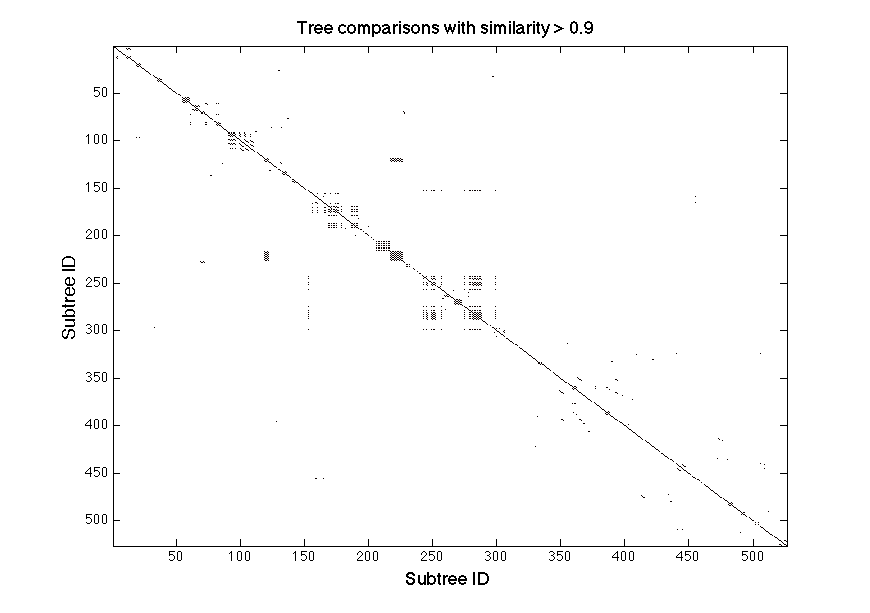
\includegraphics[width=0.45\textwidth]{figures/distmatrix-0-9.png}
\caption{Boolean matrix for the ANTLR repository indicating all pairs of
changes that have similarity greater than or equal to $\tau = 0.9$.}
\label{fig:boolmat}
\end{center}
\end{figure}

Given such a matrix, we would like to use information from the Yang
differencing algorithm to distinguish what kind of change each subtree
represents.  Three possibilities exist: a code insertion (a ``left-hole''),
code deletion (a ``right-hole''), and code mutation (a ``mismatch'').  Adding
this information to the difference matrix is important as it allows us to
further refine our view of the code evolution to distinguish code changes from
the insertion or removal of code that occurs over time. For example, when code
is being developed and grown, we expect to see a number of code insertions.
Similarly, when a mass refactoring occurs to simplify code, we would expect to
see a set of code deletions.  When a more subtle refinement occurs, such as
transposition of  code arguments or the addition of a conditional to refine
control flow, we would expect to see mismatches where the tree changes in a
way where the structural change can be thought of as a  coupled deletion and
insertion operation (such as changing a variable name in an expression).

\subsection{Anti-unification and template generation}

Once we have groups of related code snippets in the form of related subtrees,
we can seek patterns that relate changes.  For example, say we have a function
call $foo()$ where each invocation of the function uses the same parameters
(e.g, $foo(x,y)$, where $x$ and $y$ are always the same). If we add a new
parameter at the end of each call where the variable passed in differs each
time (e.g., $foo(x,y,a)$ and $foo(x,y,b)$), we would like to abstract out this
change as $foo(x,y,VAR)$, where each instance of the change replaces $VAR$
with whatever concrete variable is used at that point.  The anti-unification
algorithm is built for this purpose -- given two trees, it seeks the least-
general generalization of the pair and produces a triplet representing the
generalized tree with a metavariable introduced where the two differ, as well
as a substitution set that allows the metavariable to be replaced with the
appropriate concrete subtree necessary to reconstitute the two trees that were
antiunified.
